\documentclass[11pt]{article}

\usepackage[margin=1in]{geometry}
\usepackage{booktabs}
\usepackage{graphicx}
\usepackage{hyperref}
\usepackage{amsmath}
\usepackage{amssymb}
\usepackage{array}
\usepackage{enumitem}
\usepackage{caption}

\title{Native Nervous Interfaces for Bounded Software-Agent Command Selection}
\author{Anonymous Authors}
\date{Draft manuscript, 2026-06-14}

\begin{document}
\maketitle

\begin{abstract}
Text-only software-agent loops expose runtime state through delayed textual
observations and then ask a language model to emit free-form actions. This paper
studies a narrower mechanism: structured receptors, native state latents,
continuation memory, bounded native heads, and post-head runtime serialization
for software-agent command selection. The evaluated unit is not a general
coding agent. It is a policy package that maps a bounded
terminal/process/filesystem/time state frame to one action from a fixed
allowlisted action space. Artifact-backed evaluations include preregistered
non-sealed pressure splits, sealed-final controls, local multi-model and
multi-seed reproduction, repo-disjoint sidecar controls, bounded
recorded-candidate patch execution, and retained negative results. The
strongest command-selection capacity package completes 20/20 public-holdout
recorded-candidate executions, while a fixed no-policy first-candidate control
completes 11/20. The evidence also exposes clear limits: an identity heuristic
matches the package on one structural sidecar split, and the later learned
descriptor-runtime smoke ties its source-overlap baseline.

We additionally test bounded homeostatic persistence across fresh runtime
executions. Three HMAC-authenticated state artifacts verify successfully,
missing-key verification fails closed, task completion is preserved, and a
10-report dossier replays by hash in a distinct directory. The retained
cross-runtime audit does not support exact internal homeostatic microdynamics.
Together, these results support a bounded native nervous-interface and
homeostatic persistent-state mechanism argument. They do not establish
unbounded semantic memory, free-form shell autonomy, open-ended repair,
production autonomy, independent external replication, or an epoch-making
architecture claim.
\end{abstract}

\noindent\textbf{Scope note.} The manuscript is a bounded local artifact-chain
report. Perfect or near-perfect scores are not interpreted without measured
baselines, zero-control classification, and explicit exclusion of production
autonomy or open-ended repair claims. It does not support production autonomy,
open-ended repair, independent reproduction, or an epoch-making architecture
claim.

\section{Research Question}

The claim tested here is not that an autonomous software engineer has been
solved. The claim is that a native nervous-interface policy can improve bounded
command selection when the correct command depends on runtime-visible evidence
that text-only or partially ablated controls do not reliably use.

The experimental unit is a single decision step over a controlled state frame,
not an unrestricted shell session. A state frame contains goal metadata,
terminal deltas, process status, filesystem freshness signals, safety flags,
and candidate commands or files. The policy must choose among bounded actions
such as waiting, reading output, refreshing state, blocking a dangerous action,
or selecting one allowlisted command slot. Free-form shell synthesis, GUI
control, robotics, open-ended patch generation, and production autonomy are
outside the evaluated mechanism.

\section{Mechanism}

The implemented policy exposes runtime state through structured receptors,
forms an NSI latent state, carries bounded continuation memory, and selects
native action fields through explicit heads rather than through model-generated
JSON. We use ``native'' in this operational sense: the learned objective predicts
internal targets, routes, action classes, command slots, file slots, confidence,
and inhibition scores; only after those heads fire does the runtime serialize the
selected head output into an external action. The mechanism therefore differs
from a prompt-only agent whose primary objective is to emit a textual action
object.

Concretely, each decision follows the same six-stage path:
\begin{enumerate}[leftmargin=*]
  \item \textbf{Receptors.} The runtime builds a structured state frame from
  bounded terminal, process, filesystem, time, goal, and safety fields.
  \item \textbf{Latent encoding.} Candidate-command, candidate-file,
  continuation, and receptor features are encoded into the package's NSI state.
  \item \textbf{Native heads.} Explicit heads select an internal target, route,
  action type, command slot, file slot, confidence, and inhibition signal.
  \item \textbf{Hard receptor priority.} Safety, stale-file, unread-stderr, and
  unread-stdout receptors can override unsafe or premature learned actions
  before external execution.
  \item \textbf{Authorization.} A bounded debug-cortex action is executable only
  if it passes confidence, allowlist, file-candidate, and dangerous-command
  gates.
  \item \textbf{Serialization.} The runtime materializes one bounded motor
  action from the selected heads; escalation without an authorized cortex action
  becomes a safe wait rather than free-form JSON generation.
\end{enumerate}

This architecture is intentionally mixed: neural heads provide the selectable
state-to-action policy, while safety and serialization gates enforce the
bounded action contract. The paper's claim is therefore a mechanism claim about
this bounded native-head package and its ablations, not a claim that every
runtime decision is unconstrained or purely neural. Figure~\ref{fig:nsi-architecture}
shows the top-level mechanism and Figure~\ref{fig:receptor-head-path} shows the
receptor-to-head decision path. All figures are backed by editable Mermaid/DOT
and draw.io source files; the PDFs included here are generated artifacts rather
than hand-edited screenshots.

\begin{figure}[ht]
\centering
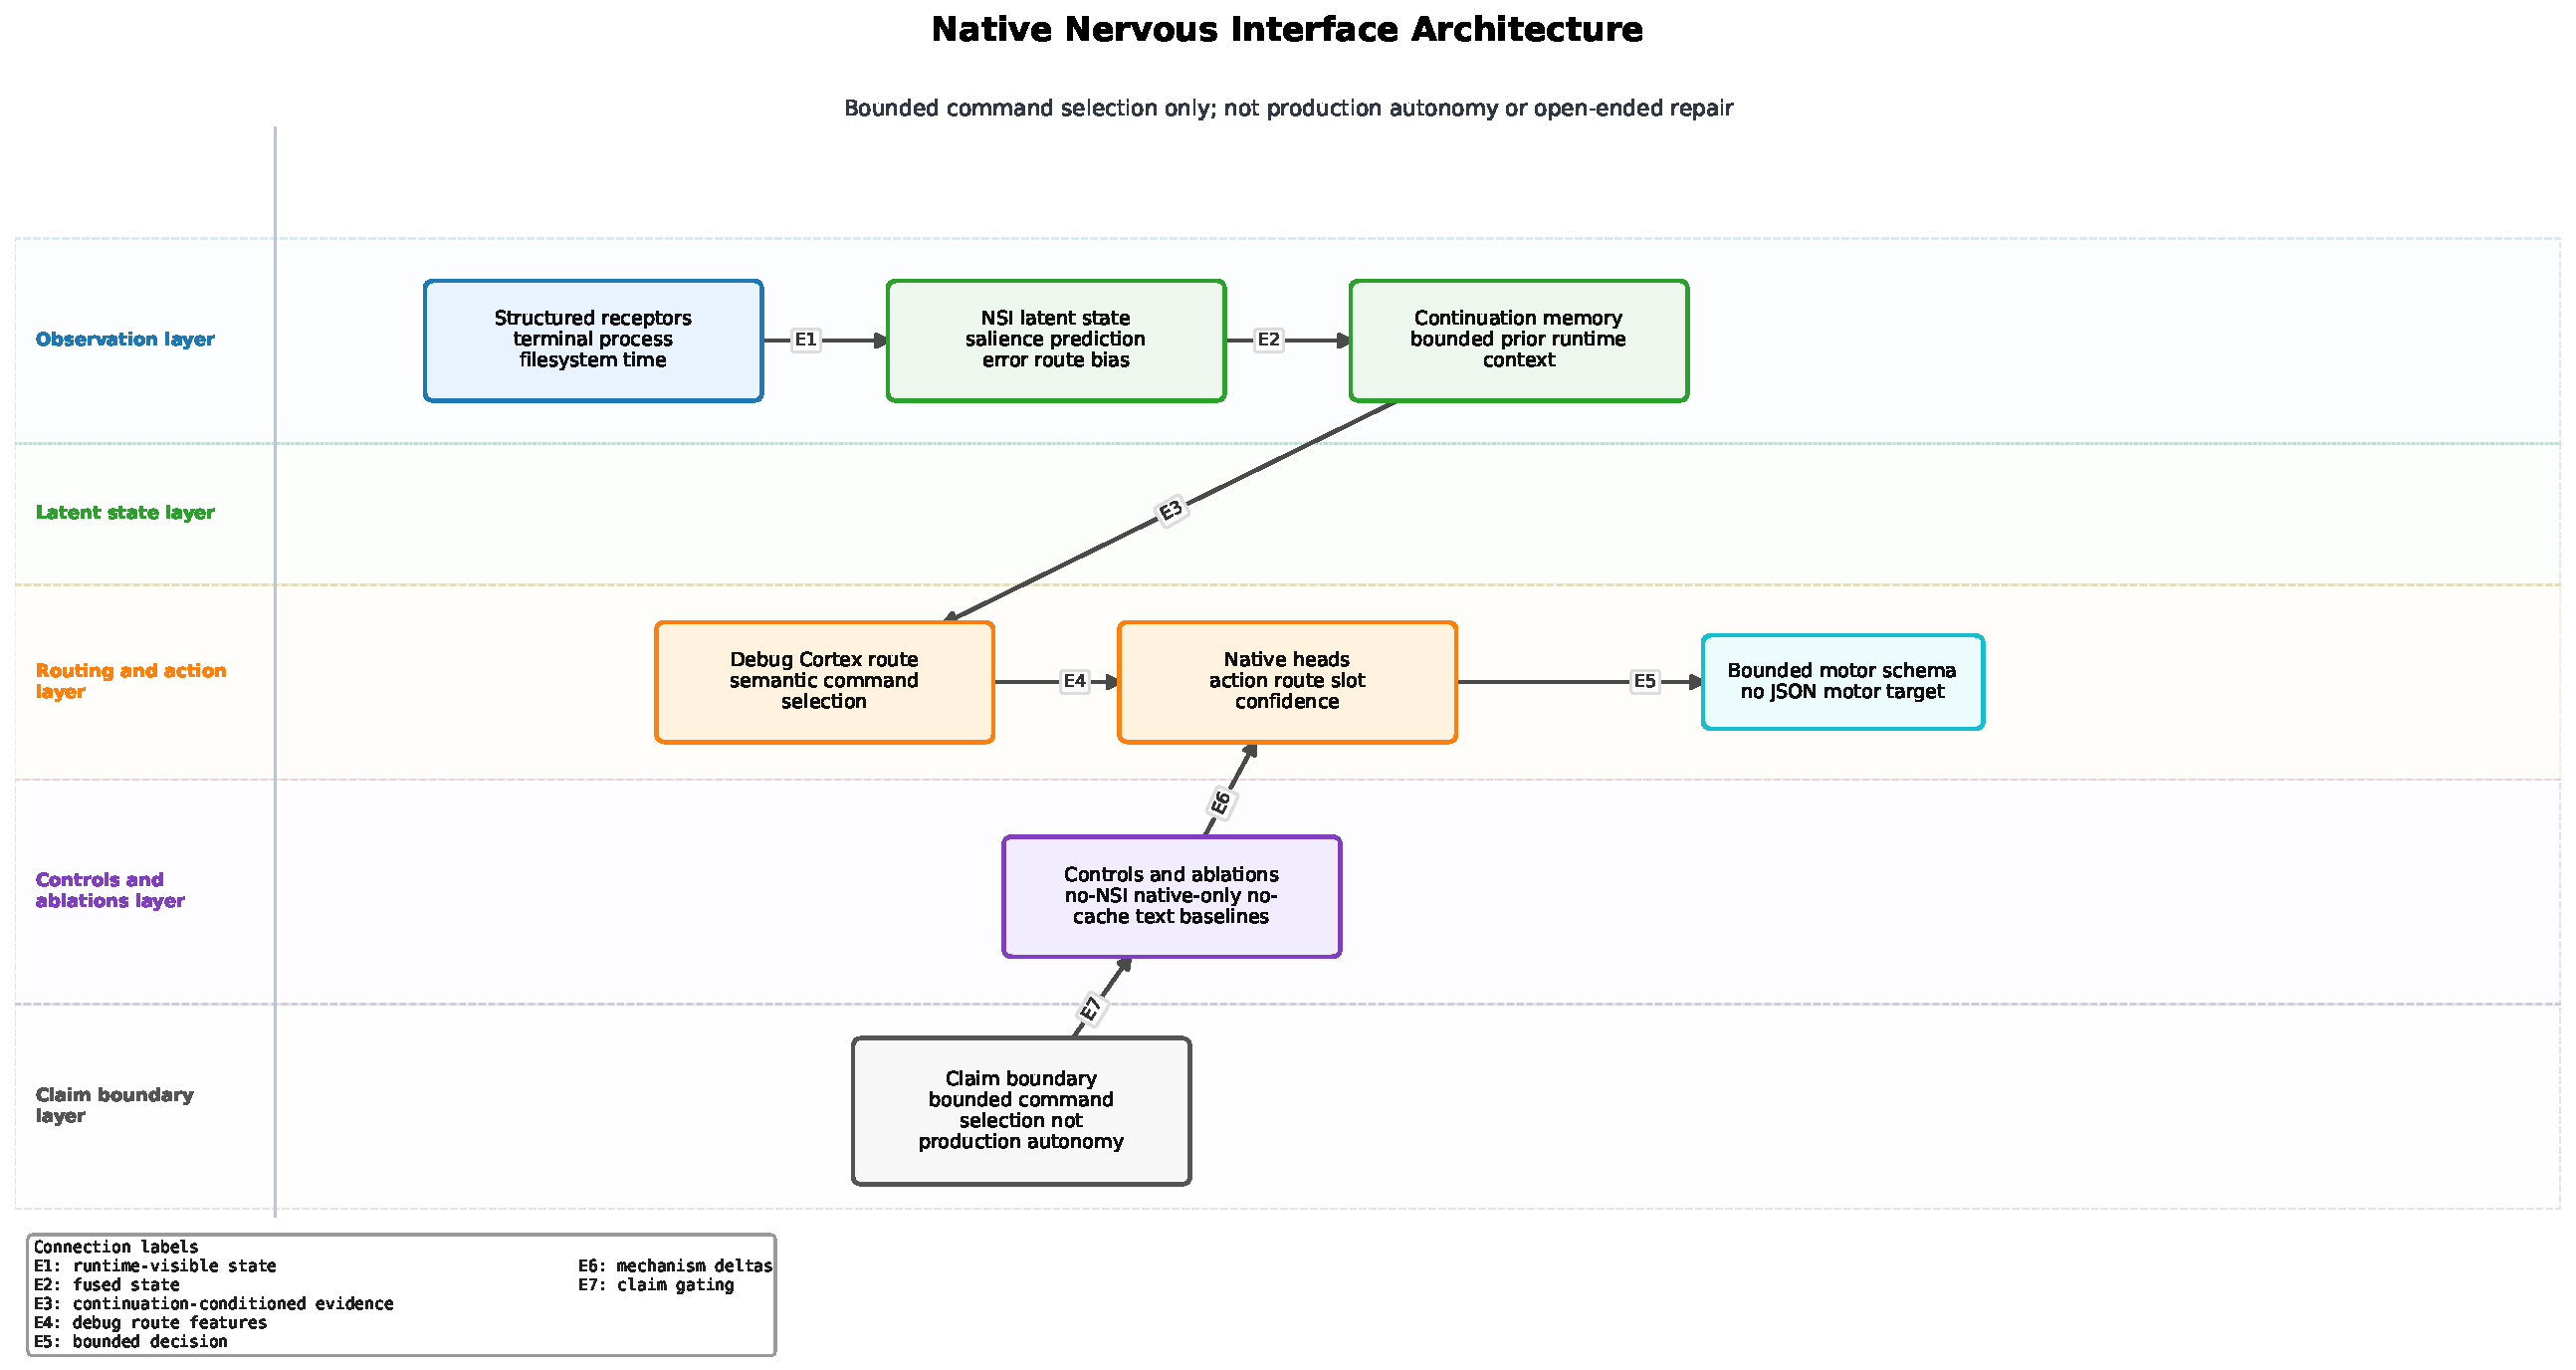
\includegraphics[width=\linewidth]{figures/nsi-architecture.pdf}
\caption{Native nervous-interface architecture used for bounded command
selection.}
\label{fig:nsi-architecture}
\end{figure}

\begin{figure}[ht]
\centering
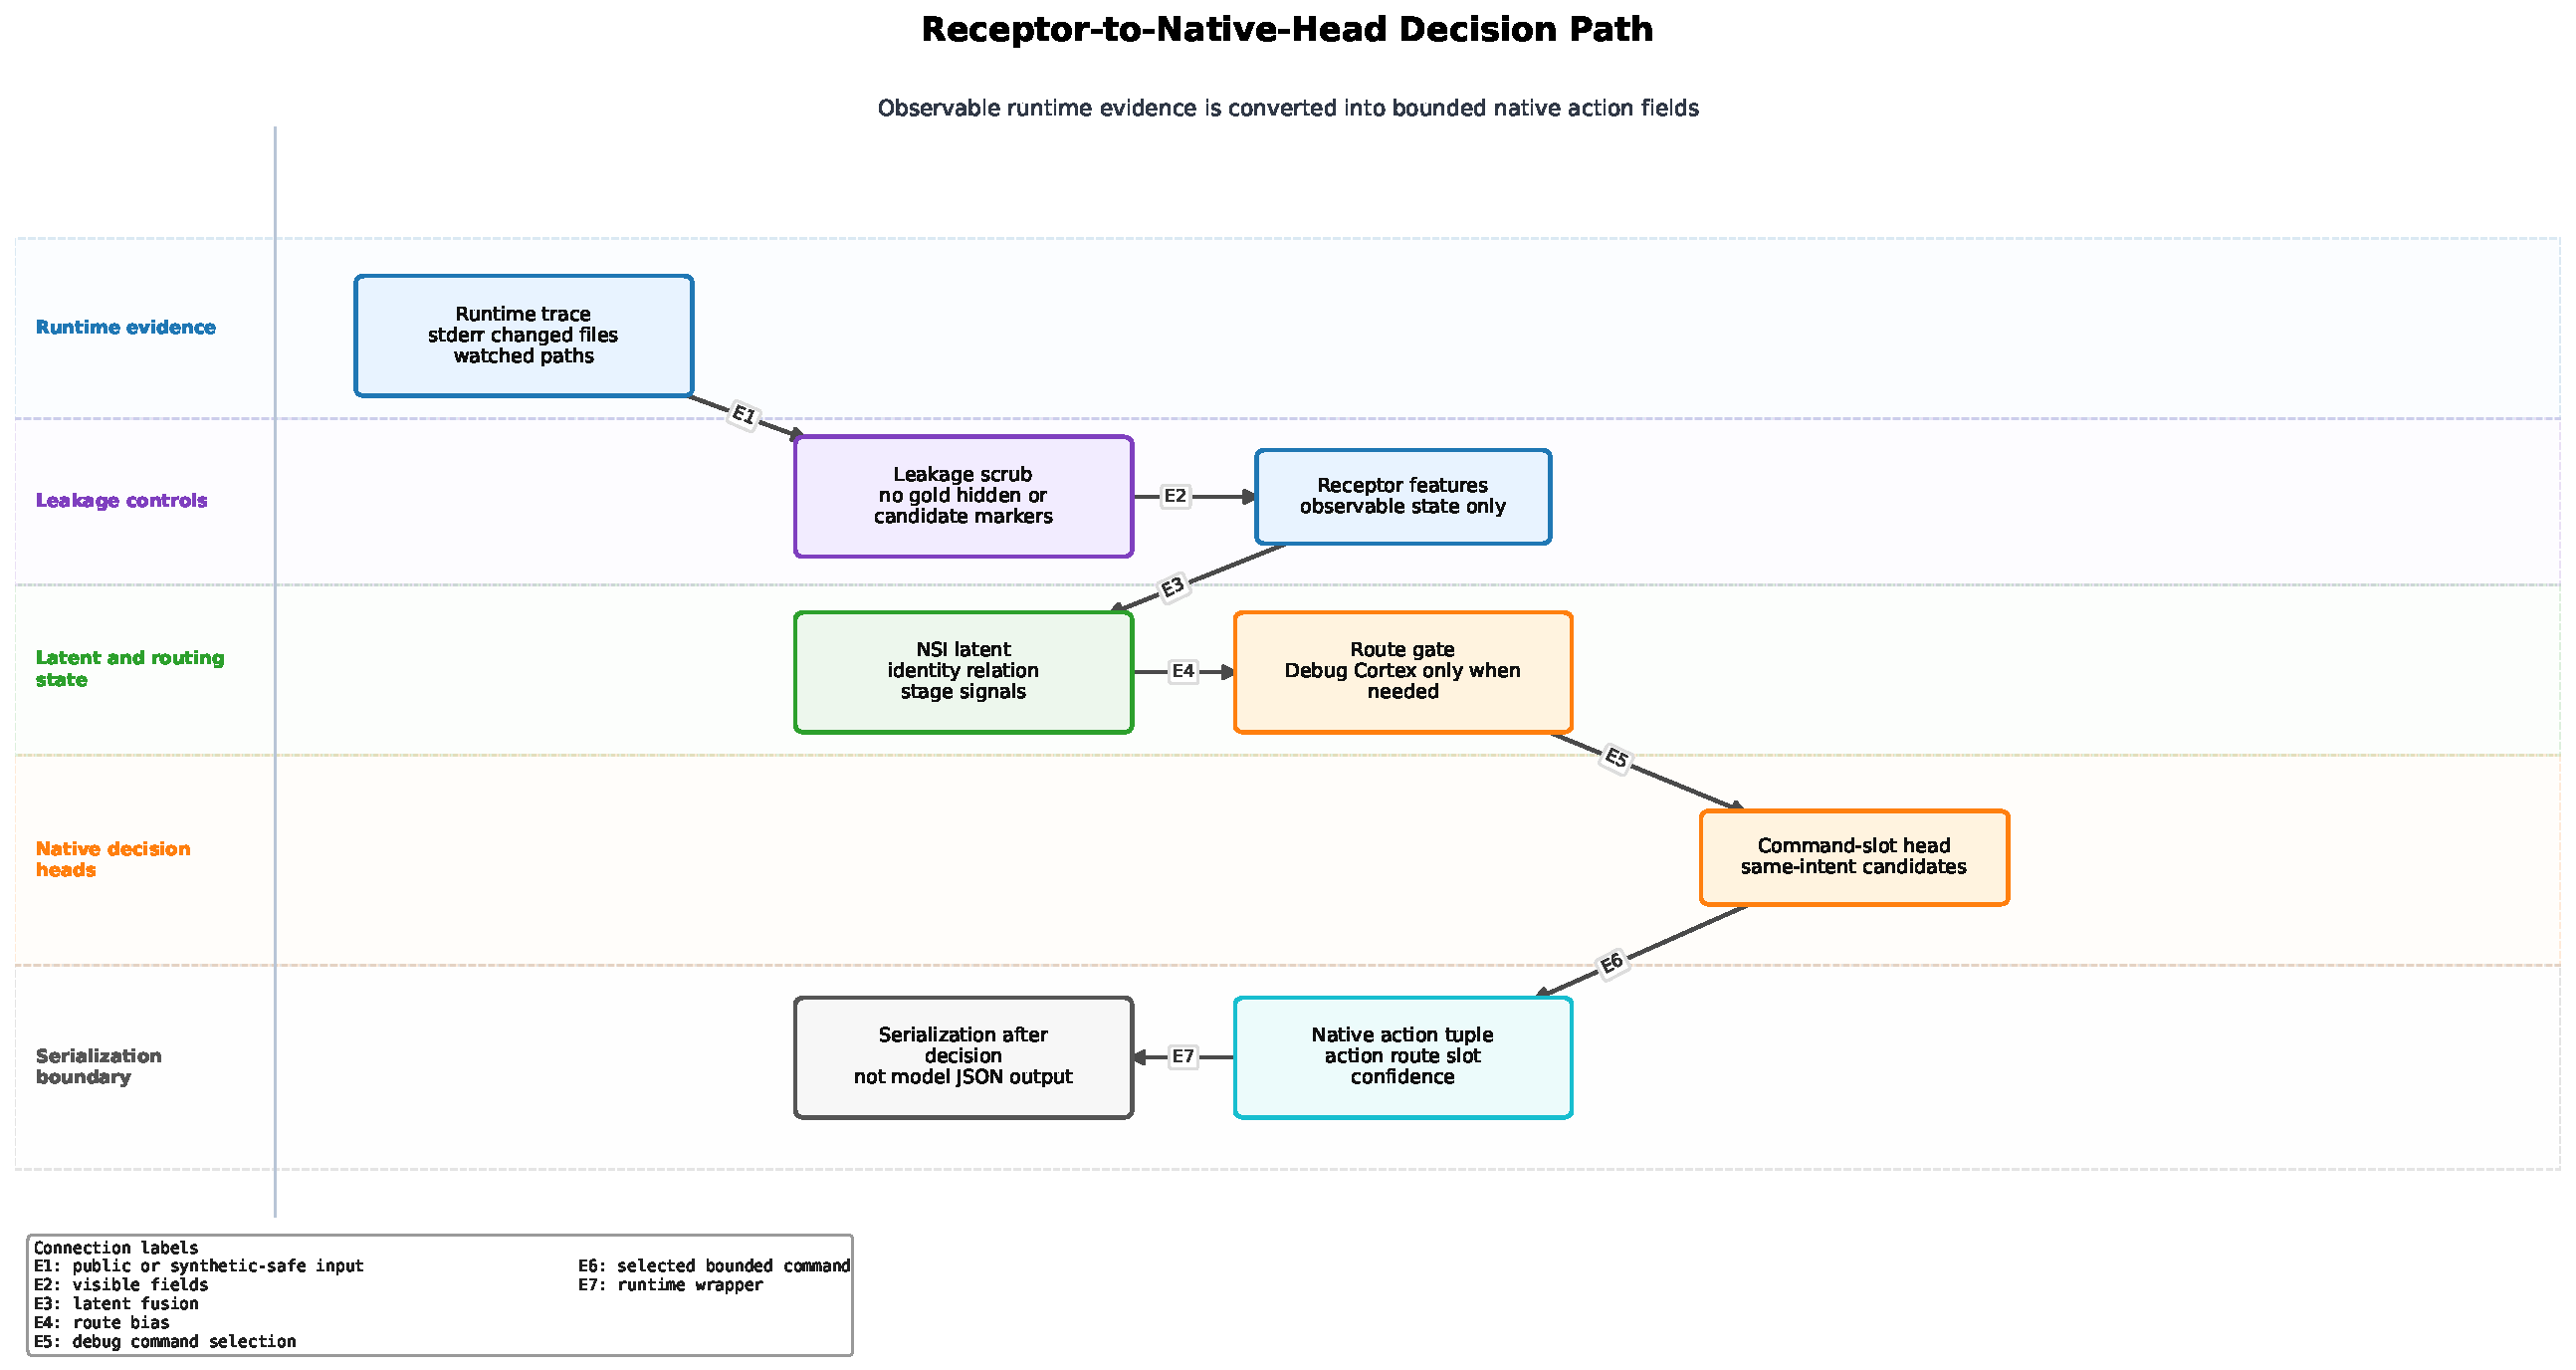
\includegraphics[width=\linewidth]{figures/receptor-to-native-heads.pdf}
\caption{Receptor-to-native-head path. Serialization occurs after native-head
selection and is not the model objective.}
\label{fig:receptor-head-path}
\end{figure}

\section{Bounded Homeostatic Persistence Evidence}

The latest mechanism-specific evidence tests whether bounded package/config
homeostatic state can survive fresh runtime execution rather than whether a
single process can merely retain an in-memory cache. Across the recorded fresh
runtime family, HMAC-authenticated persistent state transfers across bounded
executions, task completion remains successful, missing-key verification fails
closed, and the bounded dossier is replayed by hash in a distinct directory.
Table~\ref{tab:homeostasis-mechanism-evidence} binds the paper-facing summary to
the readiness artifact.

Homeostatic persistence is defined operationally, not biologically. The
controller tracks exponential moving averages of salience, risk, prediction
error, and visible failure; adapts a bounded surprise-wake threshold under
configured limits; can wake a bounded cortex, inhibit a risky side-effect
action, or habituate low-value repeated actions; and exports only a small
authenticated state artifact containing threshold and lifetime-adaptation
counts. The persistent artifact is scoped to the package and structured-runtime
checkpoint fingerprints and is accepted only when schema, integrity hash,
configuration fingerprint, scope fingerprint, numeric bounds, and HMAC
authenticator all verify. Thus the supported claim is persistent threshold and
adaptation-state transfer for bounded runtime control, not semantic memory,
private user memory, or arbitrary cross-task learning.

This evidence deliberately retains a failed exact-dynamics audit. Side-effect
traces and completion behavior remain usable for the bounded claim, but exact
cross-runtime internal homeostatic microdynamics do not match. The evidence also
does not establish unbounded or semantic long-term memory. External-machine
replay has not yet been run, so the result is local reproducibility rather than
independent replication.

\begin{table}[ht]
\centering
\small
\setlength{\tabcolsep}{3pt}
\caption{Bounded homeostatic persistent-state mechanism evidence and limits.}
\label{tab:homeostasis-mechanism-evidence}
\begin{tabular}{@{}>{\raggedright\arraybackslash}p{0.16\linewidth}>{\raggedright\arraybackslash}p{0.24\linewidth}>{\raggedright\arraybackslash}p{0.25\linewidth}>{\raggedright\arraybackslash}p{0.18\linewidth}@{}}
\toprule
Evidence layer & Positive result & Retained limitation & Paper use \\
\midrule
Fresh bounded runtime & 18 episodes; 114 actions; completion 1.000 & controlled tasks only & behavioral completion evidence \\
Authenticated persistence & 3 HMAC-authenticated state artifacts; missing-key control fails closed & bounded package/config state, not semantic long-term memory & persistent-state transfer mechanism \\
Cross-runtime limitation & 18 side-effect trace rows retained & exact internal dynamics mismatch; max active-threshold delta 0.008929 under limitation threshold 0.010000 & explicit negative evidence \\
Dossier replay & 10 source reports replayed by hash in a distinct directory & external-machine replay not yet run & local reproducibility, not independent replication \\
\bottomrule
\end{tabular}
\end{table}


\section{Claim Boundary}

The positive claim is restricted to bounded command selection. Let
\(A_{\mathrm{full}}\) denote full-package accuracy and \(A_b\) denote a measured
baseline. A mechanism delta is interpretable only when
\[
  \Delta_b = A_{\mathrm{full}} - A_b
\]
is measured on a preregistered split and the baseline is evaluable for that
split. Zero-valued controls are therefore not automatically stronger evidence;
they require the classification described in
Figure~\ref{fig:baseline-zero-tree}.

Table~\ref{tab:claim-boundary} gives the manuscript-level claim boundary. The
latest architecture-boundary artifact additionally records that bounded
mechanism claims are supported while stronger claims remain blocked by
identity-first retry, a runtime identity heuristic that can match full-package
selection on Phase2AE, strict pure-sidecar controls, and Phase2AT package
runtime delta failure. A Phase2AU task gate has been added to prevent future
learned-patch claims from being evaluated on tests that a no-policy symbolic
parser can solve directly. The current behavioral candidate now passes that
task gate and the corresponding head pretrain gate. Its Qwen2.5-0.5B capacity
package also passes a bounded command-selection runtime gate and a Phase2AU
recorded patch-candidate execution gate against a no-policy first-candidate
control on the same 20-row holdout. This remains bounded candidate evidence:
the gate checks Phase2AU package labels, rollback restoration, unauthorized
writes, oracle absence, public-repo rows, sealed-feedback absence, and no
freeform patch claim; it executes recorded candidate patches selected by the
package, but it does not prove free-form model-generated repair. A separate
descriptor observability audit verifies that learned patch-descriptor outputs
are present in runtime artifacts and match the runtime-visible repair mode, but
it blocks descriptor-generation claims because the current holdout contains only
one operation-template pair. The next required task family must therefore
include graded public-repository rows spanning multiple bounded patch operations
and templates before any learned descriptor-runtime claim is admissible. The
first Phase2AV conversion from existing Phase2AT public structural rows supplies
two operation-template pairs, but its data-health audit still blocks training
because the generated tests are parser-oracle-solvable membership checks.
Phase2AV therefore becomes a preregistered data-quality blocker before any
learned descriptor-runtime training claim. A stricter
behavioral-attribute/import public-repository task family now passes that
non-parser-oracle data-health gate on train/validation/holdout splits of
14/8/7 rows across 5/2/2 repo origins, with both
insert-import/import-restoration and replace-attribute/call-attribute
restoration operation-template pairs. Its pretrain gate binds descriptor split
hashes, runtime task hashes, and all three data-health reports, and marks only
small-scale smoke training as ready. This is a small-scale task-family
readiness result only. The subsequent Qwen2.5-0.5B smoke uses the correct CUDA
environment and native-head row schema, but fails postflight: validation
command-slot accuracy equals the source-overlap baseline at 0.625, descriptor
operation/template accuracy remain 0.75/0.75, and the confusion matrices show
slot-0 and insert-import majority collapse. Phase2AV therefore remains negative
learning evidence after a data-quality pass; learned descriptor-runtime deltas,
full training, packaging, sealed transfer, freeform patch generation,
open-ended repair, production autonomy, and epoch-making architecture claims
remain unsupported.

\begin{table}[ht]
\centering
\scriptsize
\setlength{\tabcolsep}{2pt}
\caption{Claim boundary for the bounded mechanism paper.}
\label{tab:claim-boundary}
\begin{tabular}{@{}>{\raggedright\arraybackslash}p{0.13\linewidth}>{\raggedright\arraybackslash}p{0.36\linewidth}>{\raggedright\arraybackslash}p{0.34\linewidth}@{}}
\toprule
Status & Claim & Paper use \\
\midrule
supported & Bounded native-head Debug Cortex command selection & Main positive mechanism claim \\
supported & NSI latent contribution versus no-NSI on semantic-required controls & Mechanism delta claim with measured ablations \\
supported & Local multi-model and multi-seed robustness for bounded command selection & Robustness layer; independent reproduction remains separate \\
supported with caveat & Phase2T sealed transfer after zero-control root-cause audit & Usable only with non-sealed baseline-feasibility sanity; not a strong architecture claim \\
supported with caveat & Runtime-visible natural sidecar dependency on repo-disjoint public traces & Supported for bounded command-slot selection; strict pure-sidecar causality remains unproven \\
supported with caveat & Package-level structural sidecar runtime under residual budget pressure & Supported as non-sealed package-runtime sidecar evidence; raw runtime identity heuristic still matches full on this split \\
supported with caveat & Bounded symbolic patch proposal runtime & Supported only for text-membership public-repo holdout24; not freeform patch generation \\
unsupported & Superiority over identity-first verification retry & Phase2AA strict retry ties full and blocks this upgrade \\
unsupported & Learned bounded patch package-runtime delta & Phase2AT loaded package tied the no-policy symbolic structural runner at 256/256 \\
supported with caveat & Phase2AU policy-required package/no-policy runtime and patch-candidate execution delta & The 73-row behavioral task gate, 33/20 head pretrain gate, Qwen0.5B identityrefv2 smoke/holdout, package gate, 20-row command-selection runtime gate, and Phase2AU-specific 20-row bounded patch-candidate execution gate pass; use only as bounded capacity evidence, because Qwen1.5B is locally throughput-blocked and learned freeform repair remains unproven \\
unsupported & Multi-template learned patch-descriptor runtime generation & Phase2AU runtime artifacts contain learned descriptor outputs, but the descriptor observability audit sees only one insert-import/import-restoration operation-template pair; a graded multi-operation task family is still required \\
supported with caveat & Phase2AV non-parser-oracle multi-template descriptor-runtime task family & The behavioral attribute/import public-repo train/validation/holdout splits pass data-health plus hash-bound pretrain/launch gates with two operation-template pairs and non-parser-oracle generated tests, but only at 14/8/7 rows \\
unsupported & Phase2AV learned descriptor-runtime full-training/package readiness & The Qwen0.5B smoke on the newer behavioral attribute/import split fails postflight: command-slot accuracy ties source-overlap at 0.625 and descriptor operation/template heads remain at 0.75/0.75; full training, package, sealed evidence, and learned runtime-delta claims are blocked \\
unsupported & Production autonomy, unrestricted shell use, open-ended repair & Explicitly excluded from Paper B \\
unsupported & Epoch-making architecture status & Requires independent reproduction, broader open-ended repair, safety analysis, and stronger baselines \\
\bottomrule
\end{tabular}
\end{table}


\begin{figure}[ht]
\centering
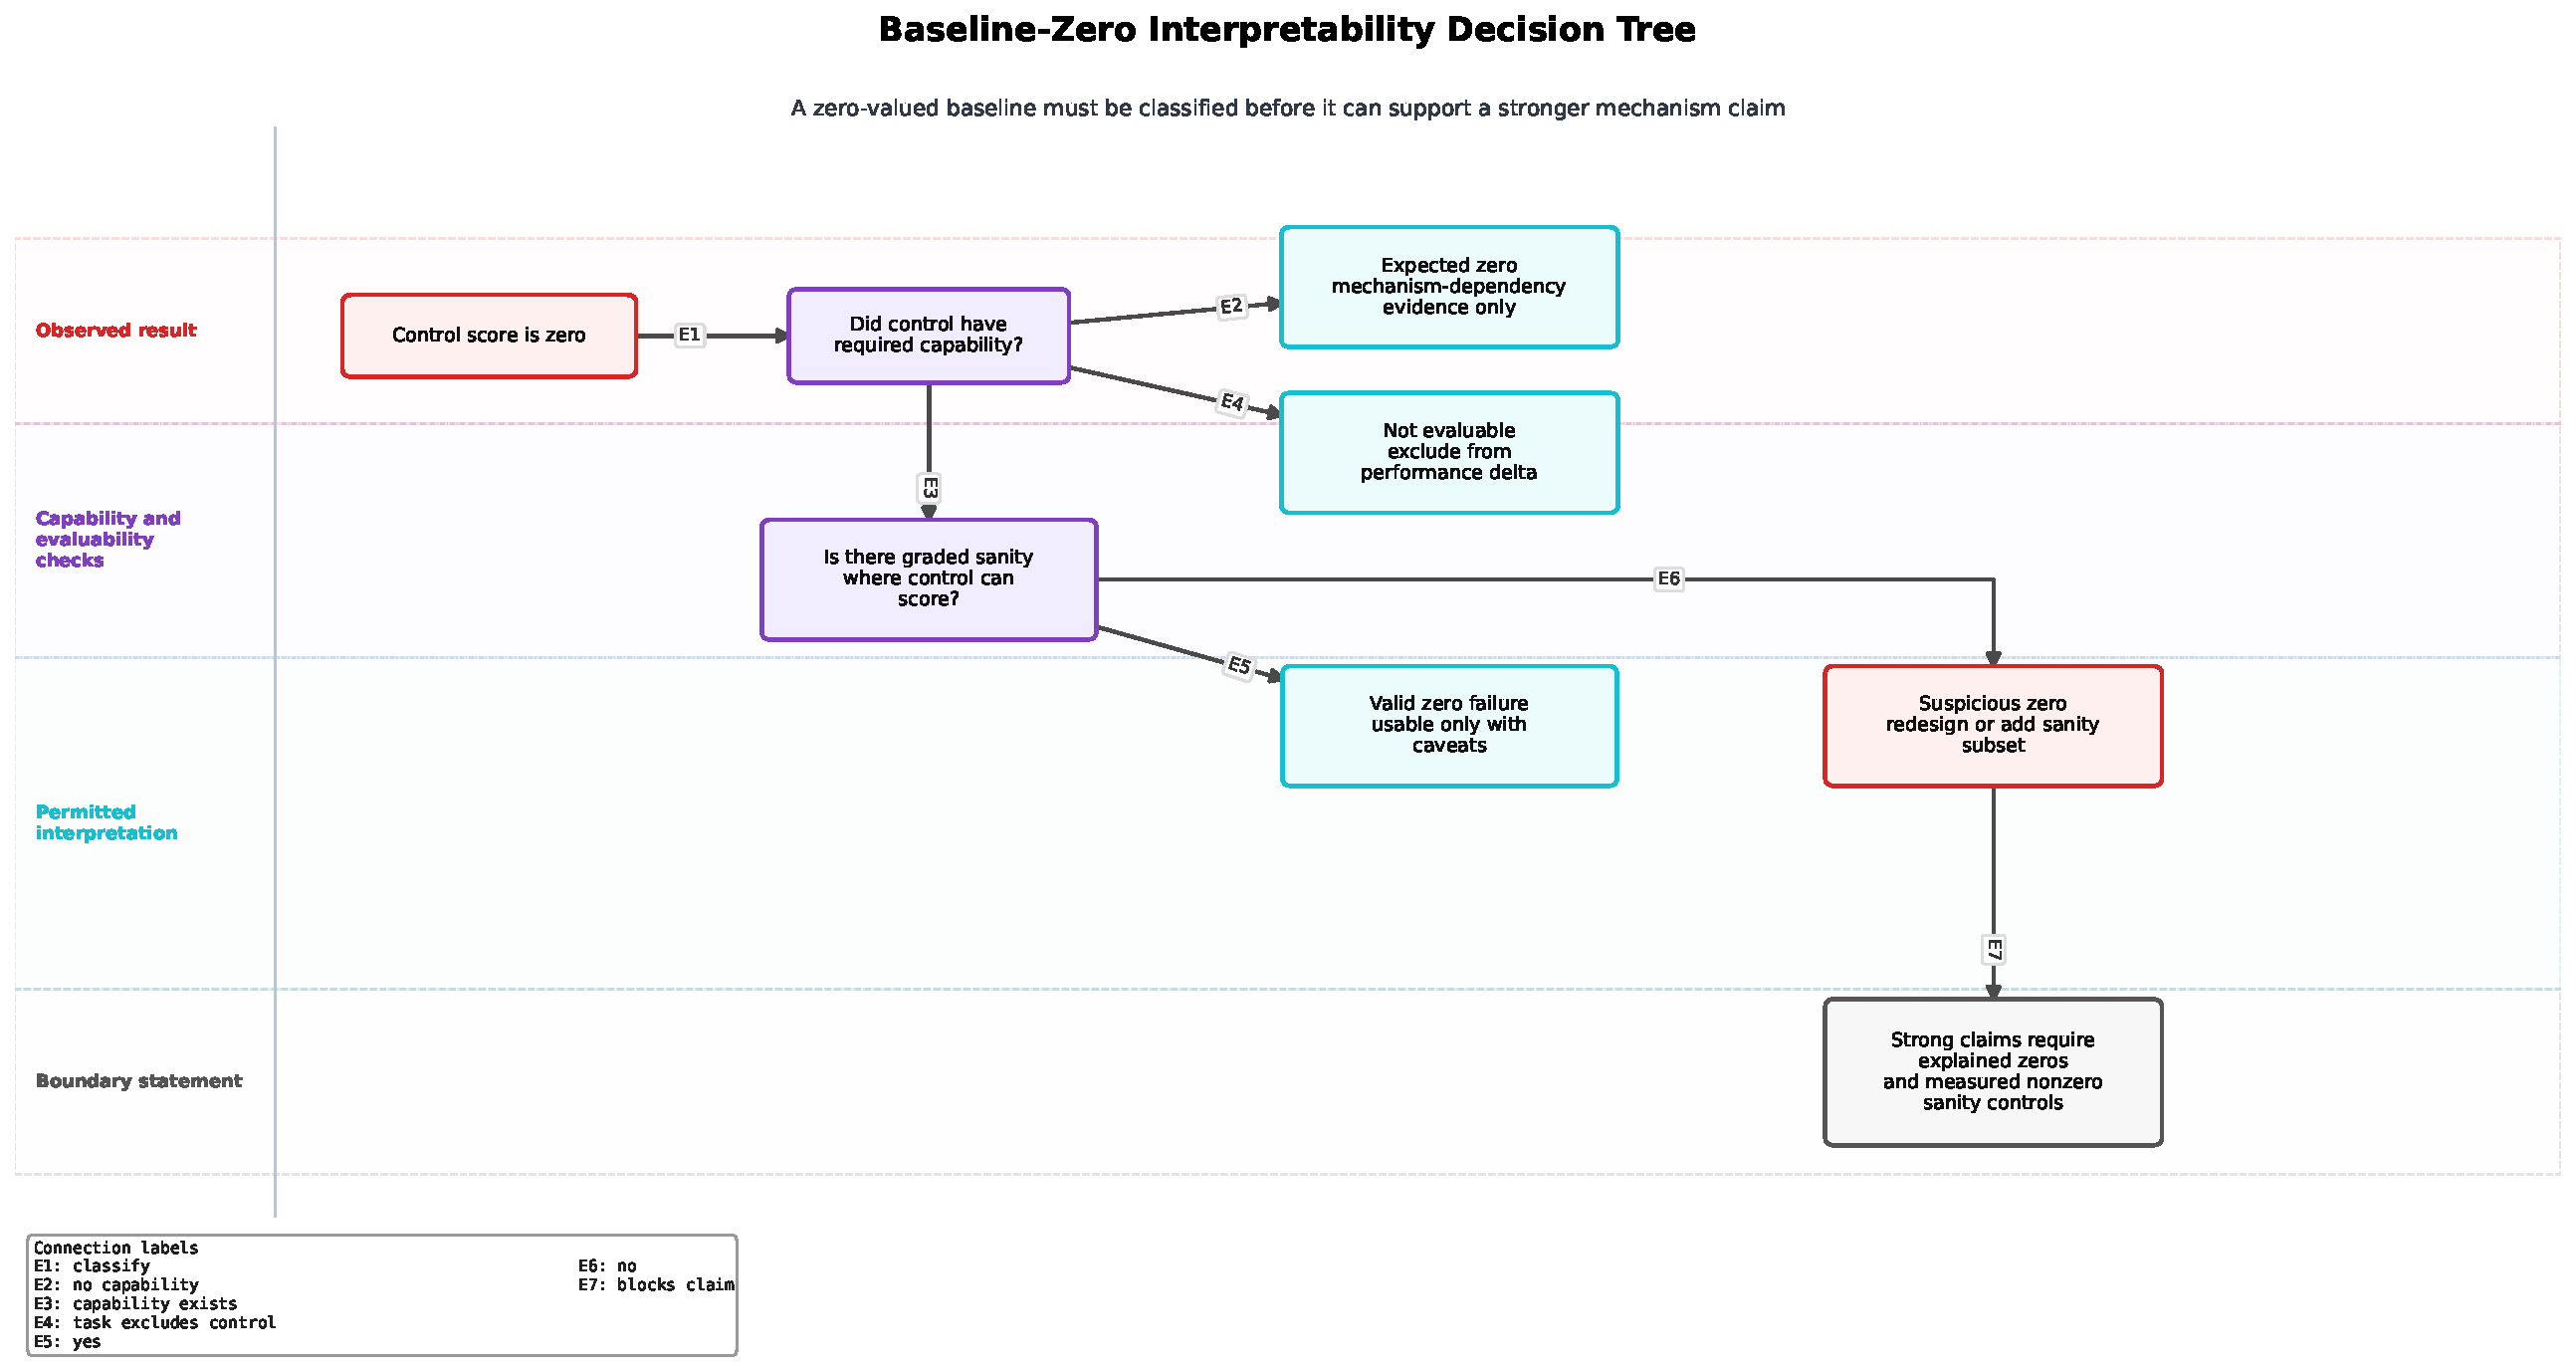
\includegraphics[width=\linewidth]{figures/baseline-zero-decision-tree.pdf}
\caption{Decision tree for interpreting zero-valued controls. A zero control
may be expected, valid failure evidence, non-evaluable, or suspicious.}
\label{fig:baseline-zero-tree}
\end{figure}

\section{Evidence Ladder}

The evidence ladder begins with public relation-key pressure, continues through
sealed cross-model transfer, adds public breadth and dynamic pytest traces, and
then tests the public-repair split across local 3B/7B models and three seeds per
model. Phase2T adds a later sealed-transfer and non-sealed baseline-feasibility
sanity layer for the all-zero-control problem. Earlier negative phases remain
part of the evidence boundary rather than being reinterpreted as positive
results.

Table~\ref{tab:positive-evidence} summarizes the positive evidence layers.
Phase2AE is included as package-level sidecar runtime evidence, not as evidence
that learned heads outperform an explicit runtime identity heuristic.

\begin{figure}[ht]
\centering
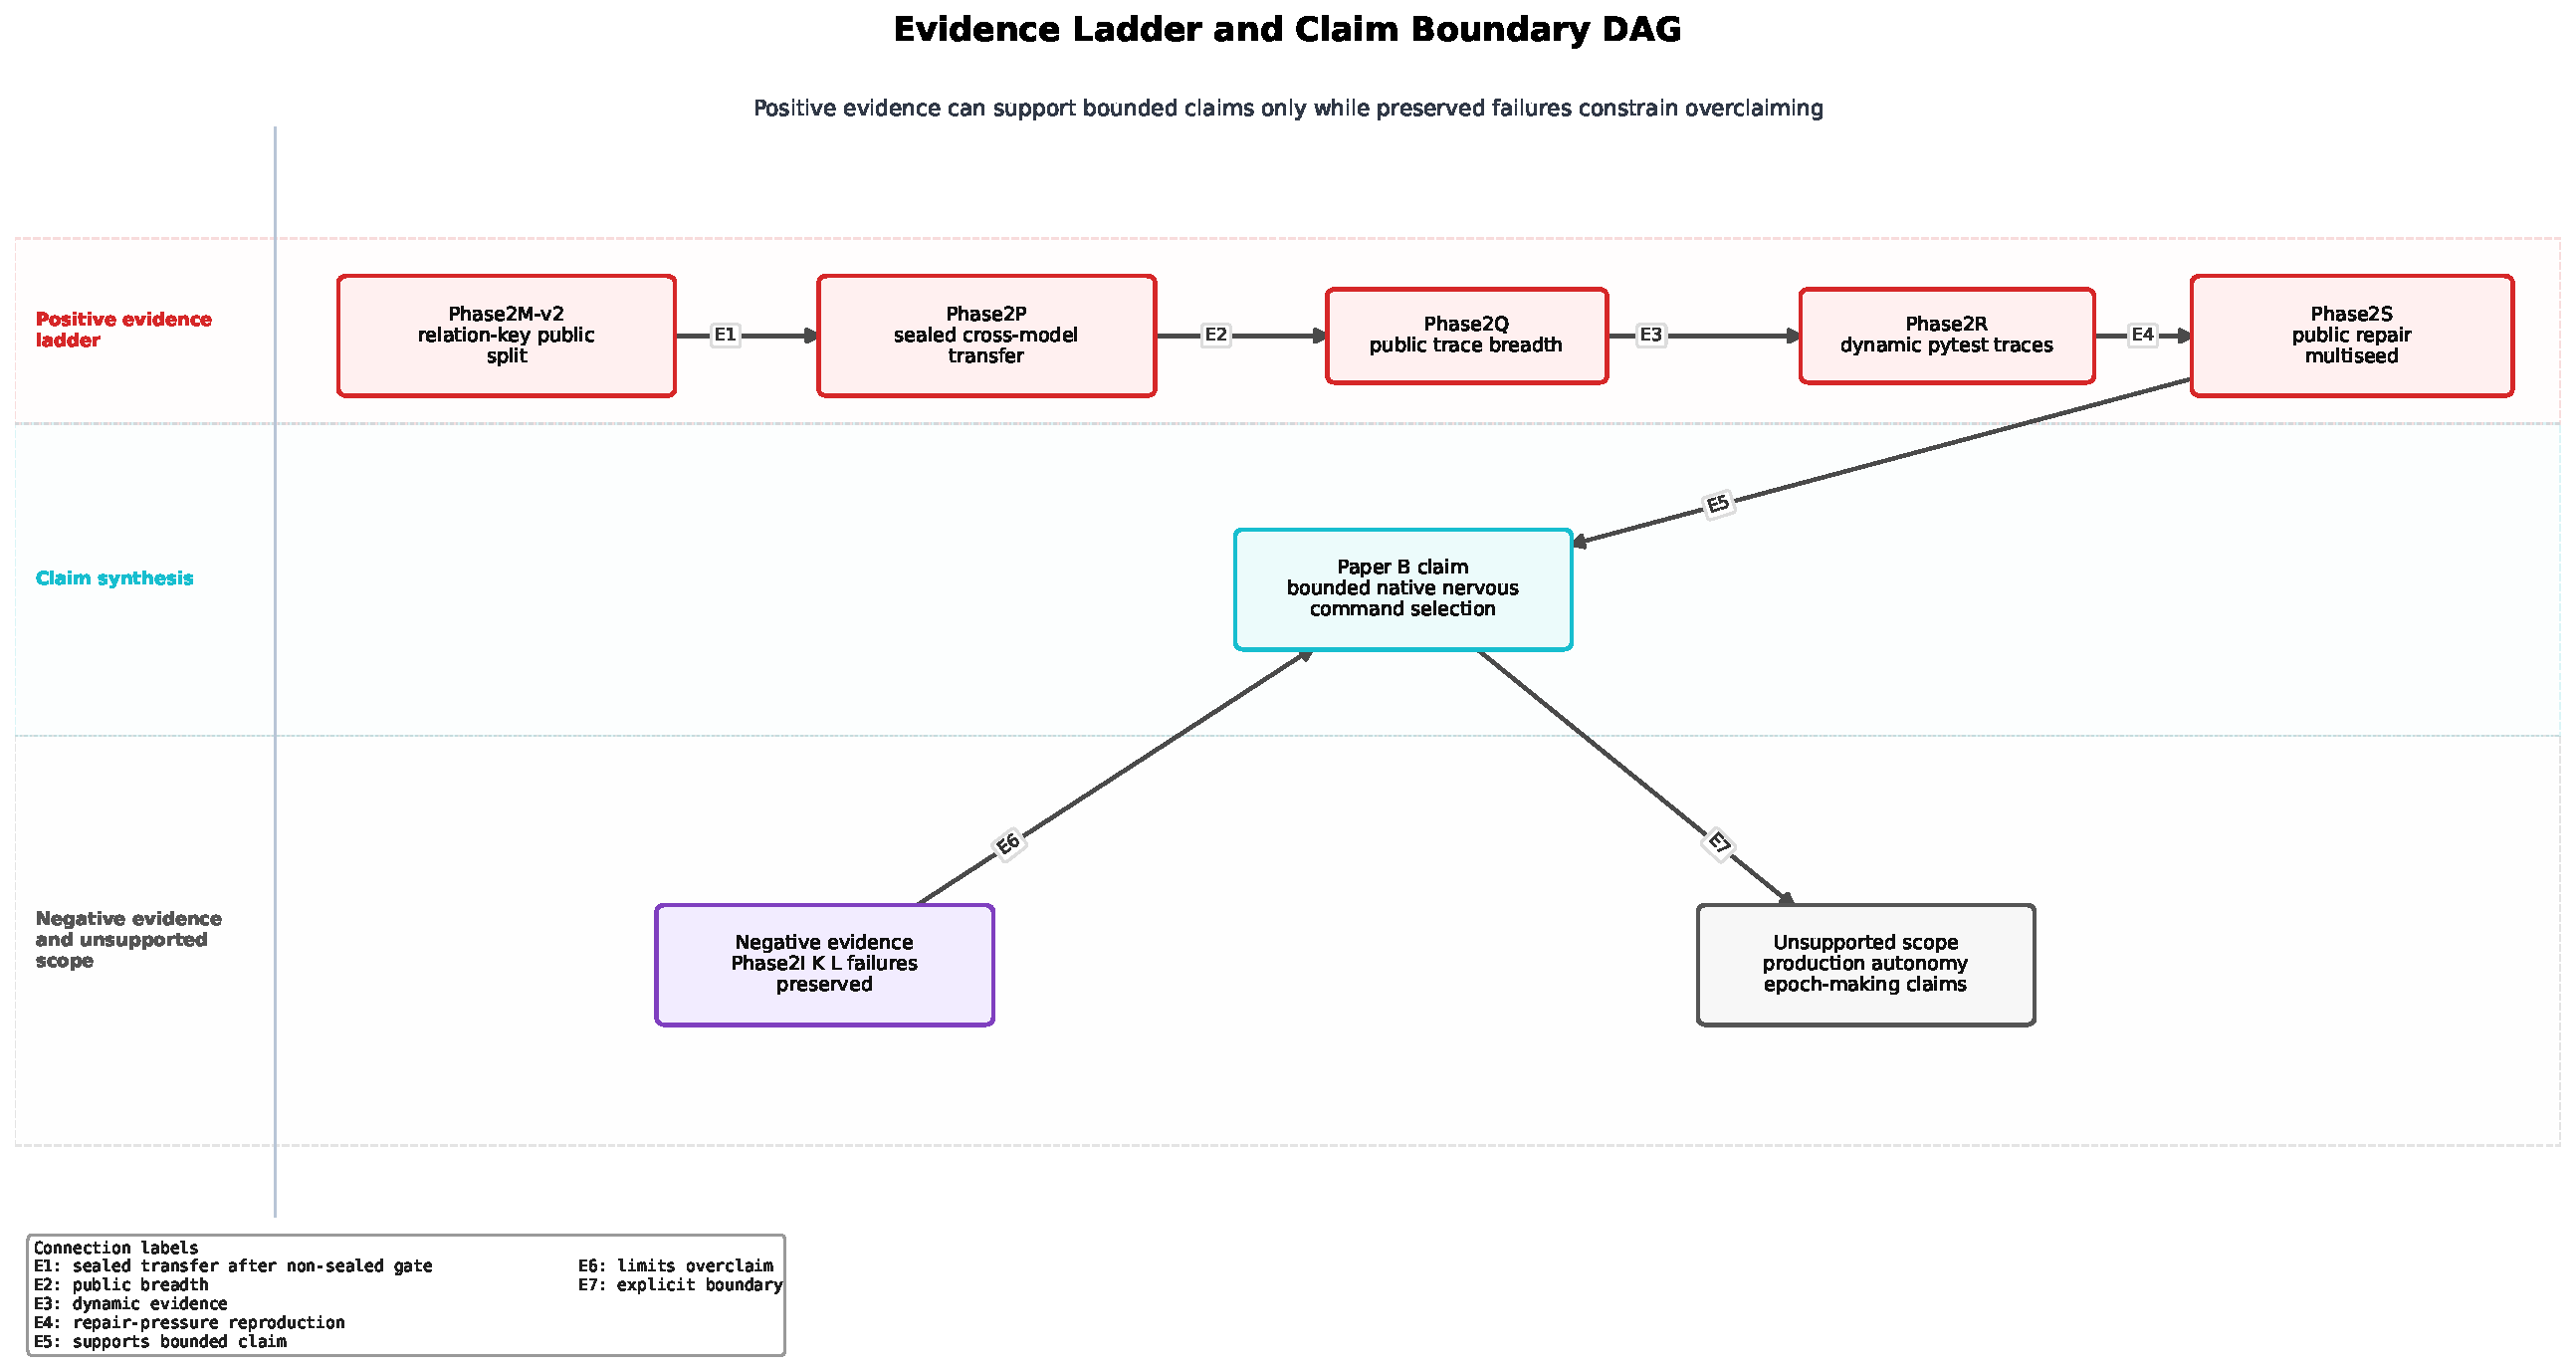
\includegraphics[width=\linewidth]{figures/evidence-ladder.pdf}
\caption{Evidence ladder and boundary for Paper B. Phase2S adds local
same-family multi-seed public-repair reproduction, while production autonomy,
general open-ended repair, and epoch-making architecture claims remain outside
the supported scope.}
\label{fig:evidence-ladder}
\end{figure}

\begin{table}[ht]
\centering
\scriptsize
\setlength{\tabcolsep}{2pt}
\caption{Positive evidence matrix for bounded command-selection claims.}
\label{tab:positive-evidence}
\begin{tabular}{@{}>{\raggedright\arraybackslash}p{0.10\linewidth}>{\raggedright\arraybackslash}p{0.16\linewidth}>{\raggedright\arraybackslash}p{0.21\linewidth}>{\raggedright\arraybackslash}p{0.13\linewidth}>{\raggedright\arraybackslash}p{0.22\linewidth}@{}}
\toprule
Layer & Non-sealed full & Source/native pressure & Sealed full & Boundary \\
\midrule
Phase2M-v2 & 1.000 & source 0.371; native 0.367 & 1.000 & single local 7B run \\
Phase2P & reuses Phase2M-v2 family & no-NSI max 0.688; native max 0.000 & min 1.000; 15/15 gates & local cross-model transfer, not independent reproduction \\
Phase2Q & 1.000 & source 0.348; native 0.332 & 1.000 & static public trace breadth \\
Phase2R & 1.000 & source 0.344; native 0.371 & 1.000 & dynamic pytest traces, still command selection \\
Phase2S & holdout min 0.905; mean 0.907 & source-delta min 0.531; no-NSI-delta min 0.535 & separate final-eval evidence only & 3B/7B x 3 seeds on non-sealed public repair split; same-family, not production autonomy \\
Phase2T & holdout 1.000 & source 0.406; no-NSI 0.313; slot-head 0.156 & 0.953 & all-zero sealed controls require baseline-feasibility caveat; strong architecture claim remains blocked \\
Phase2AA & 1.000 across 3B plus 1.5B seeds 13/17/23 & fixed no-policy 0.395; no-NSI 0.395; delta 0.605 & not used & bounded candidate-selection runtime delta; identity-first verification retry ties full and blocks stronger claim \\
Phase2AE package runtime & package runtime 45/45; full 1.000 & policyless 0.000; erased 0.000; wrong 0.000; identity heuristic 1.000 & not used & package structural sidecar closes residual budget-pressure gap; no learned-head superiority over explicit identity heuristic \\
\shortstack[l]{Phase2AM\\Phase2AP} & natural full min 0.991 & source 0.527; erased max 0.518; wrong max 0.402 & not used & natural repo-disjoint sidecar dependency reproduced across models/seeds; strict pure-sidecar causality remains blocked by residual controls \\
\shortstack[l]{Phase2Z\\Phase2AQ} & symbolic patch runtime 24/24 & source 0.500; model-source 0.500 & not used & bounded symbolic text-membership patch proposal runtime; not freeform model-generated patch repair \\
Phase2AU capacity package & Qwen0.5B val 1.000; holdout 1.000; runtime command 20/20; patch execution 20/20 & source/no-policy 0.550; holdout source-delta rows 9; command and execution delta 0.450 & not used & identityrefv2 capacity package beats fixed no-policy control for bounded command selection and Phase2AU-gated recorded patch-candidate execution; descriptor outputs are observable but single-template only; Qwen1.5B local throughput blocked and freeform patch generation remains unproven \\
Phase2AV pretrain gate & smoke failed & train/val/holdout 14/8/7 rows; 5/2/2 repos; descriptor/runtime/head hashes bound; two operation-template pairs; non-parser-oracle tests & not used & data-quality positive only; Qwen0.5B smoke tied source-overlap and failed descriptor gates, so no learned runtime-delta, full-training, or package result \\
\bottomrule
\end{tabular}
\end{table}


\section{Controls and Baselines}

The control matrix includes the full package, no-NSI latent ablations,
native-head-only/no-cache controls, continuation-only controls, prompt-only and
ReAct text baselines, and measured source-overlap baselines. Figure~\ref{fig:control-matrix}
summarizes their role.

Table~\ref{tab:baseline-zero-summary} records how zero-valued controls are
interpreted. Table~\ref{tab:negative-evidence} keeps failed and bounded phases
inside the paper rather than hiding them.

\begin{figure}[ht]
\centering
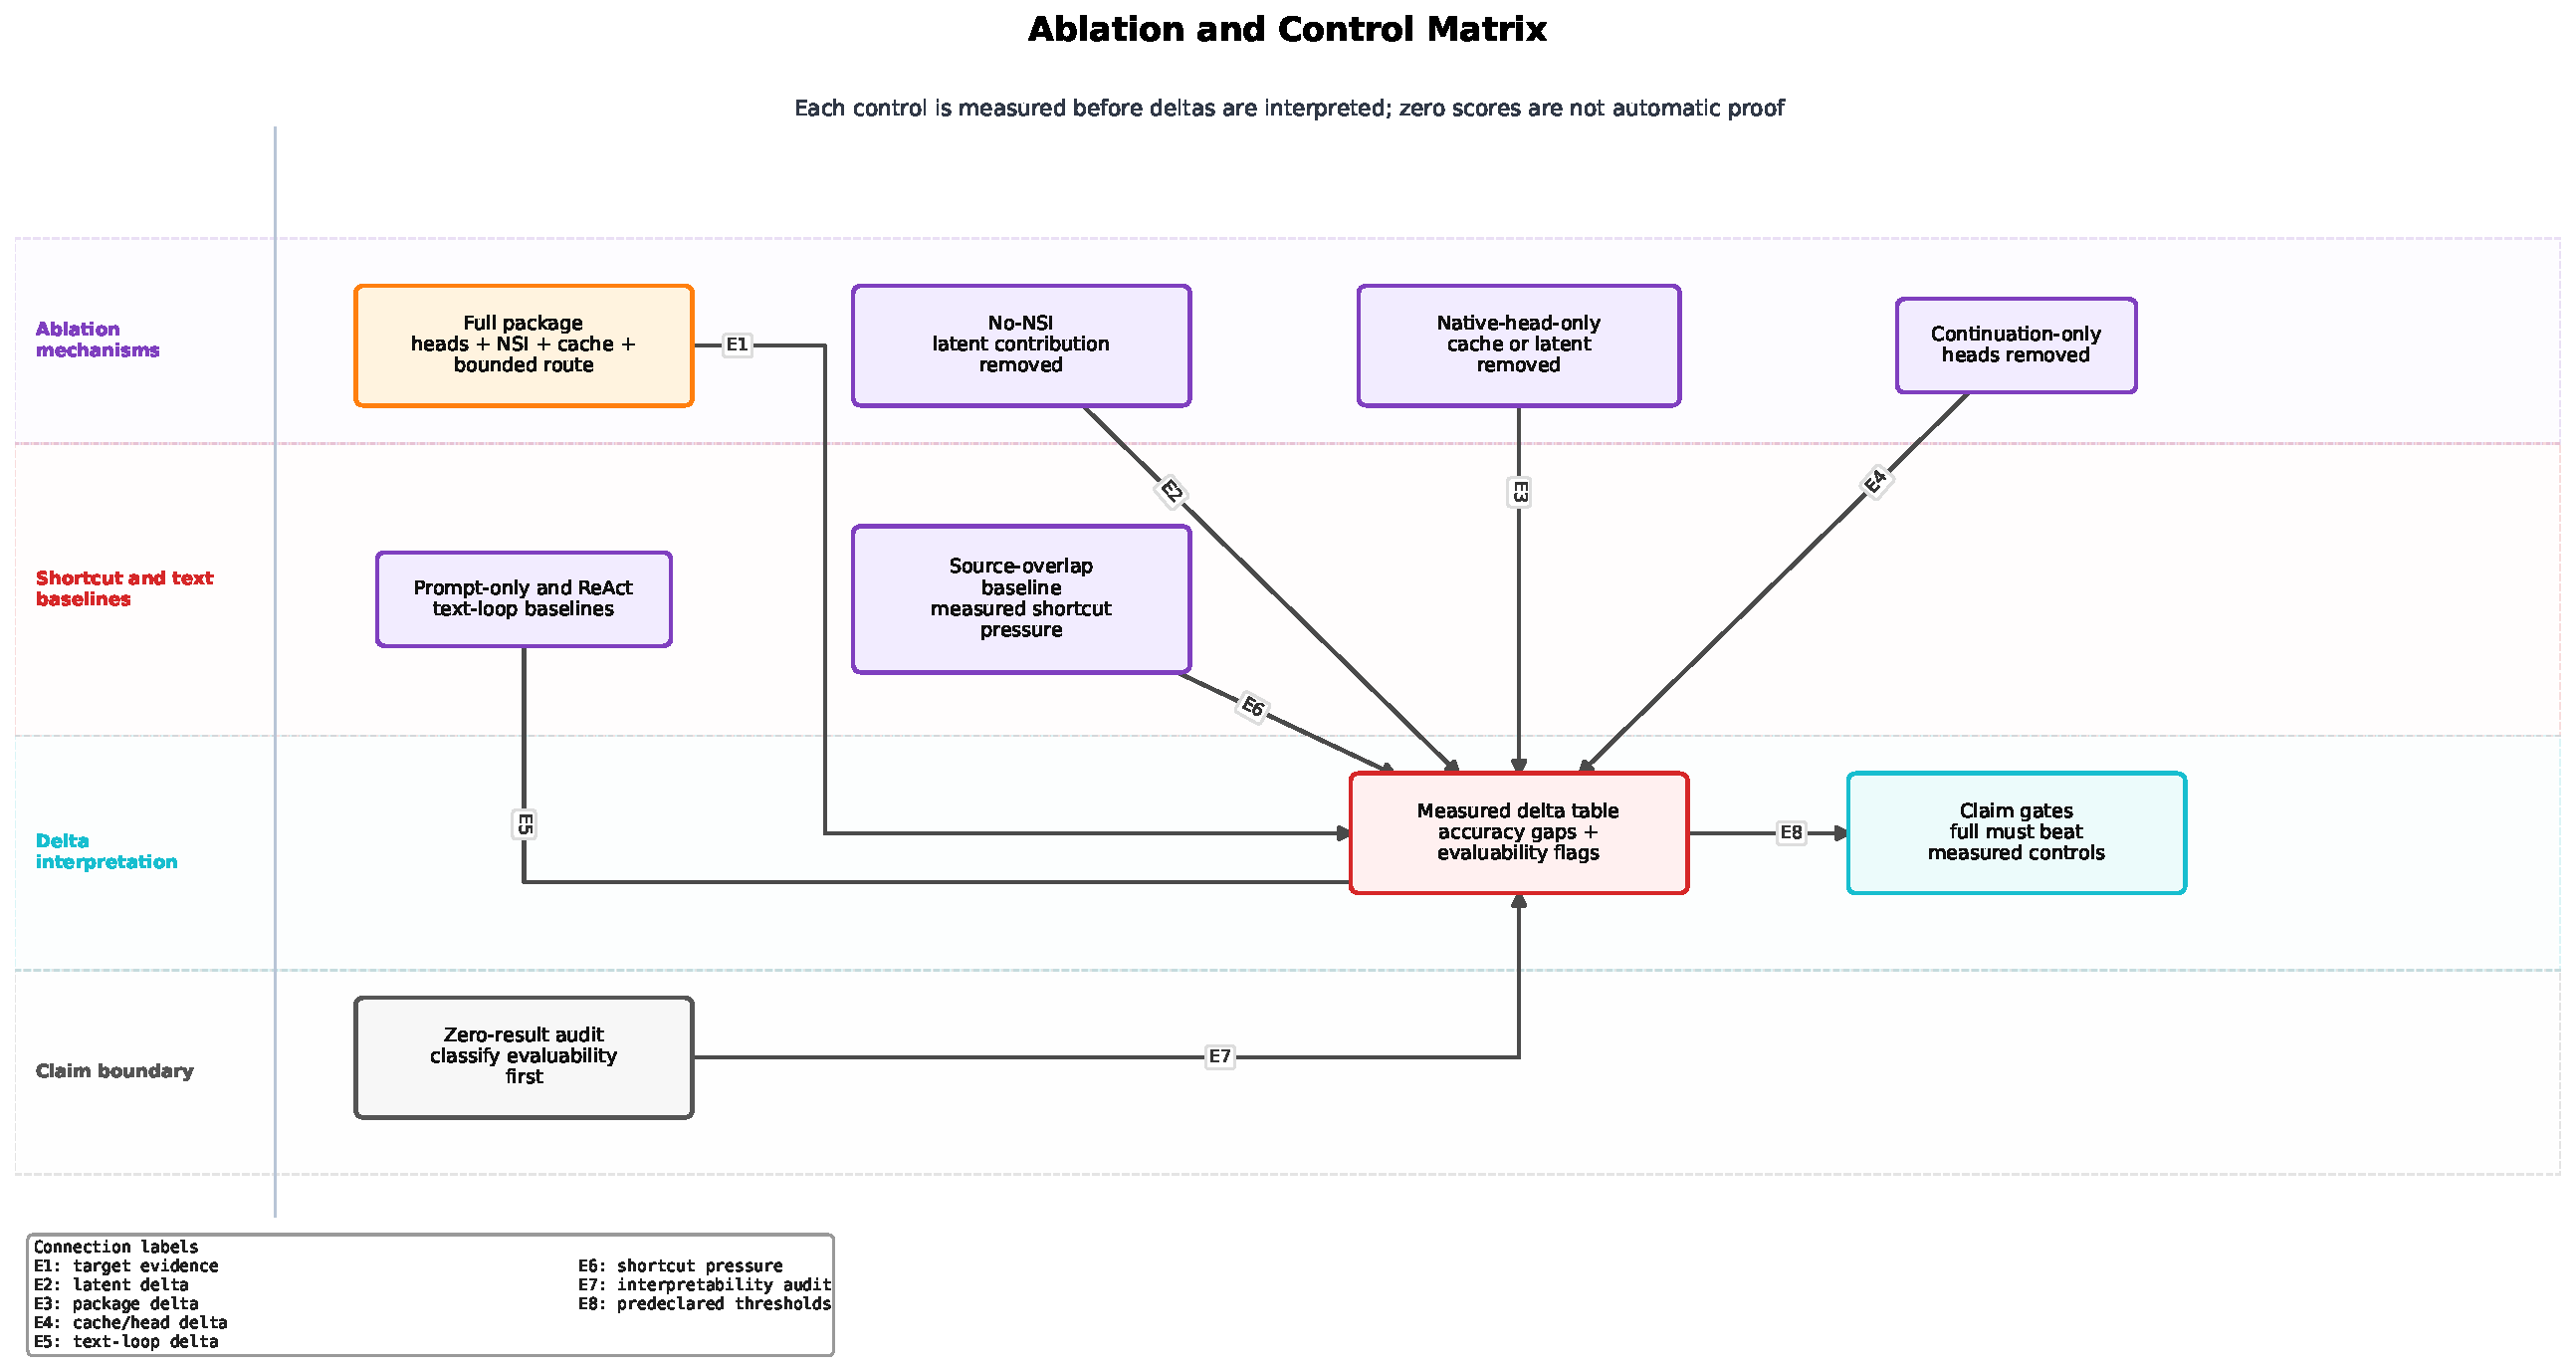
\includegraphics[width=\linewidth]{figures/ablation-control-matrix.pdf}
\caption{Ablation and control matrix. Each stronger claim requires measured
deltas against the relevant control rather than relying on a naked zero.}
\label{fig:control-matrix}
\end{figure}

\begin{table}[ht]
\centering
\footnotesize
\setlength{\tabcolsep}{3pt}
\caption{Interpretability audit for zero-valued controls.}
\label{tab:baseline-zero-summary}
\begin{tabular}{@{}>{\raggedright\arraybackslash}p{0.10\linewidth}>{\raggedright\arraybackslash}p{0.16\linewidth}>{\raggedright\arraybackslash}p{0.21\linewidth}>{\raggedright\arraybackslash}p{0.13\linewidth}>{\raggedright\arraybackslash}p{0.22\linewidth}@{}}
\toprule
Phase & Native and no-NSI both zero & Full zero & Zero categories & Claim blocker \\
\midrule
Phase2M-v2 & no & no & expected missing capability; valid zero failure & classified; not standalone broad proof \\
Phase2Q & yes & no & expected missing capability; valid zero failure & classified; requires non-sealed feasibility context \\
Phase2R & no & no & expected missing capability; valid zero failure & classified; not standalone broad proof \\
Phase2L & yes & yes & expected missing capability; valid zero failure & negative sealed-transfer evidence only \\
Phase2P & no & no & expected missing capability; valid zero failure & classified; local transfer only \\
Phase2T & yes & no & expected missing capability; valid zero failure & no strong claim from sealed all-zero controls; mitigated by non-sealed baseline-feasibility sanity \\
\bottomrule
\end{tabular}
\end{table}


\begin{table}[ht]
\centering
\tiny
\setlength{\tabcolsep}{1pt}
\caption{Negative and bounded evidence retained as claim boundary.}
\label{tab:negative-evidence}
\begin{tabular}{@{}>{\raggedright\arraybackslash}p{0.13\linewidth}>{\raggedright\arraybackslash}p{0.36\linewidth}>{\raggedright\arraybackslash}p{0.34\linewidth}@{}}
\toprule
Phase & Observed limit & Interpretation \\
\midrule
Phase2I & full equals no-NSI on sealed v3; latent split lacked command identity & not evidence for semantic-required NSI latent necessity \\
Phase2J initial smoke & model matched source-overlap baseline & blocked full training until source-overlap-hard redesign \\
Phase2K sealed gate & full did not beat native-head-only on sealed v3 & non-sealed continuation pressure did not transfer \\
Phase2L sealed gate & all six mechanisms completed 0/64 & sealed transfer failure, not positive continuation proof \\
Phase2M synthetic-safe smoke & synthetic plumbing split exposed candidate-slot leakage risk & infrastructure smoke only, not claim-bearing evidence \\
Phase2T sealed controls & no-NSI, native-head-only, continuation-only, prompt-only, and ReAct all completed 0/64 & bounded sealed claim requires explicit zero-root audit plus non-sealed baseline-feasibility sanity; not epoch-making architecture evidence \\
Phase2AA strict retry control & identity-first bounded verification retry completed 256/256, tying full package & evidence supports bounded candidate selection versus fixed/no-NSI controls, but not superiority over retry-based verification policy \\
Phase2AE runtime identity heuristic & package-level structural sidecar runtime completed 45/45, but raw runtime identity heuristic also solved 45/45 before text ablation & closes package-runtime sidecar gap while blocking any claim that learned heads outperform an explicit runtime identity heuristic \\
Phase2AP strict pure-sidecar controls & stable bounded sidecar controls pass, but strict erased-residual and pure-sidecar checks fail in some runs & supports sidecar-controlled selection with caveats; does not support pure sidecar causality or stronger architecture claims \\
Phase2Z/AQ symbolic patch runtime & bounded symbolic text-membership patch proposal succeeds on holdout24 & positive runtime evidence, but still not model-generated patch diff, diverse repair, or open-ended debugging \\
Phase2AT package runtime delta & loaded package and no-policy symbolic structural runner both completed 256/256; full-control delta 0.000 & descriptor-head and schema evidence do not yet prove learned bounded patch runtime advantage; next task must make no-policy symbolic control insufficient \\
Phase2AU policy-required runtime path & Phase2Y-to-Phase2AU conversion yields 0/128 rows; a behavioral public-repo candidate later passes the 64-row task gate with 73 rows and 9 repo origins; 33/20 head train/validation rows pass pretrain gate with split hashes; Qwen0.5B identityrefv2 smoke and holdout reach 1.000 against 0.550 source-overlap; the Qwen0.5B capacity package then reaches 20/20 runtime command-selection success and 20/20 Phase2AU-gated bounded patch-candidate execution success versus 11/20 fixed no-policy control, but Qwen1.5B local runs time out before writing progress & supports bounded capacity package/no-policy command-selection and recorded patch-candidate execution delta only; learned freeform patch generation, sealed transfer for this package, and stronger architecture claims remain unsupported, and the 1.5B throughput blocker remains negative evidence \\
Phase2AU descriptor runtime observability & learned descriptor outputs are recorded in runtime rows and match the runtime-visible repair mode, but all 20 successful rows are insert-import/import-restoration & descriptor output plumbing is observable, but multi-template descriptor-generation evidence is blocked until a graded public-repo task family spans multiple bounded patch operations and templates \\
Phase2AV initial graded descriptor-runtime gate & conversion from existing Phase2AT rows yields 256 public rows, 4 repo origins, and two operation-template pairs, but generated tests are parser-oracle-solvable & correct blocker: do not train or claim learned descriptor-runtime delta from the Phase2AT-derived rows \\
Phase2AV behavioral attribute/import smoke & non-sealed public-repo train/validation/holdout runtime tasks pass non-parser-oracle multi-template data-health and hash-bound launch gates, but Qwen0.5B smoke reaches command-slot 0.625 versus source-overlap 0.625 and descriptor operation/template 0.75/0.75 & fixes the parser-oracle data-design blocker at small scale, then fails learned smoke postflight through slot-0 and insert-import majority collapse; full training, package, sealed-transfer, freeform patch-generation, open-ended repair, and production-autonomy evidence remain blocked \\
\bottomrule
\end{tabular}
\end{table}


\section{Data and Validation}

Claim-bearing data must be non-sealed, leakage-scrubbed, and accompanied by
repo-disjoint splits, source-overlap baselines, postflight gates, and fixed
hashes. Sealed v3 is final-evaluation only and is not allowed to influence
training, sampling, seed selection, or failure-feedback design.

\begin{figure}[ht]
\centering
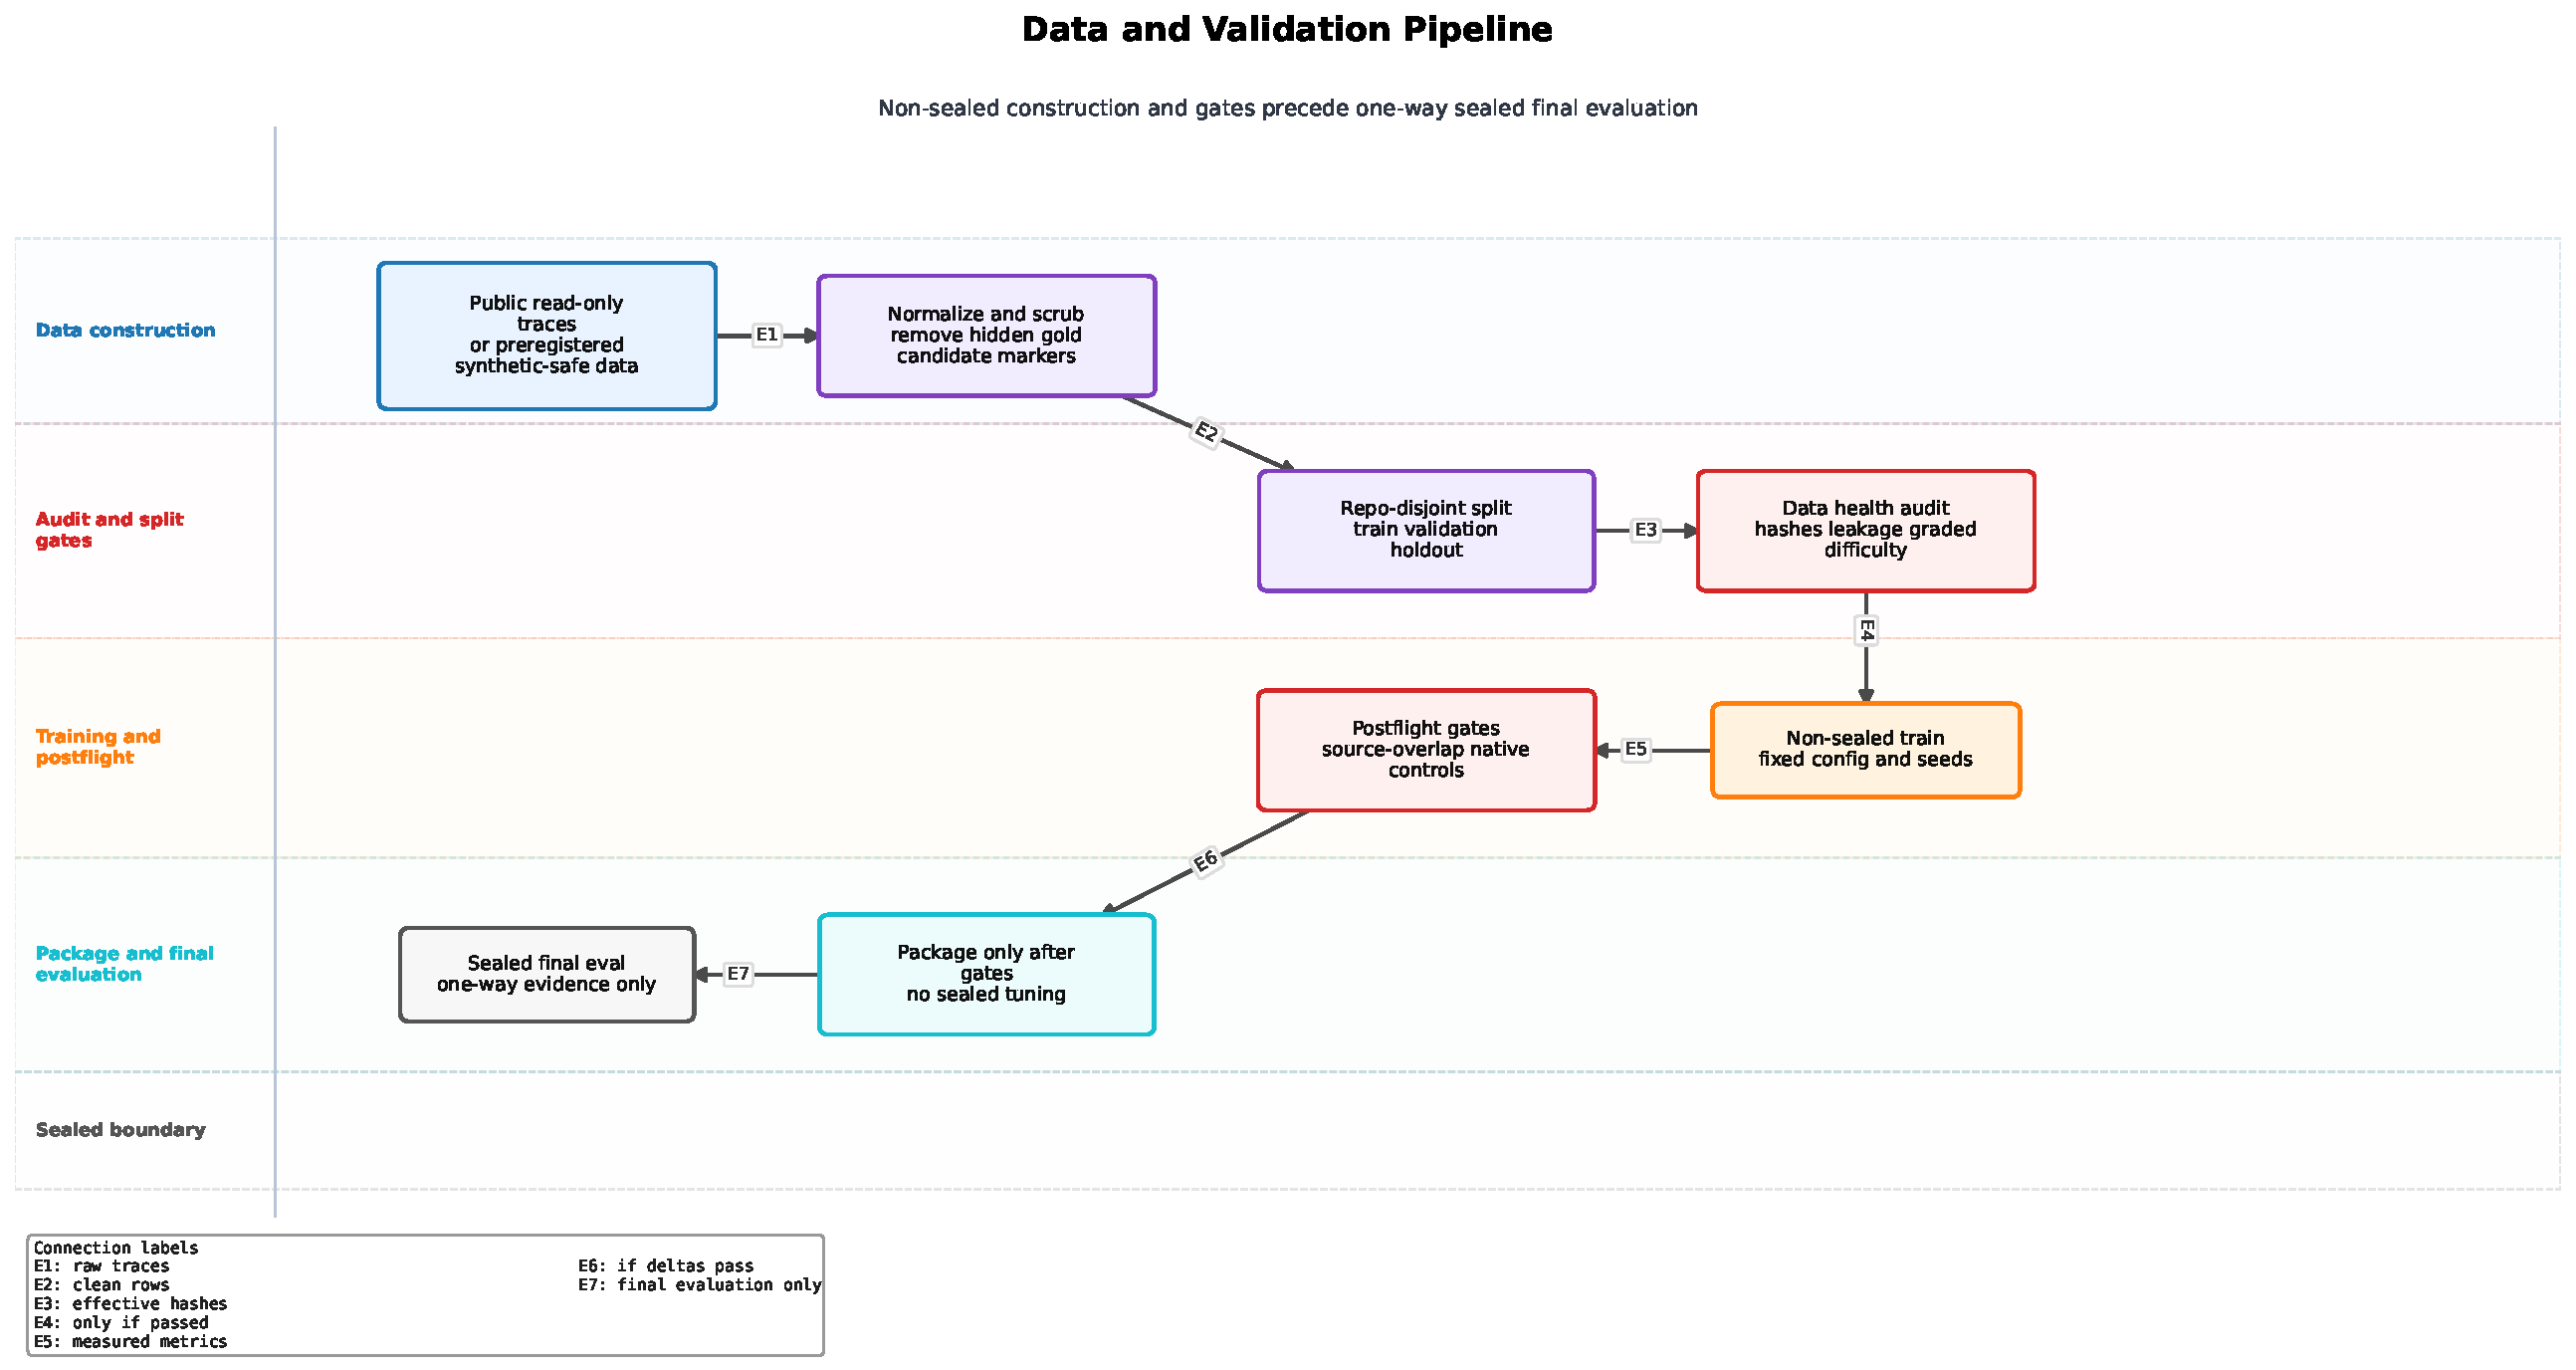
\includegraphics[width=\linewidth]{figures/data-validation-pipeline.pdf}
\caption{Data and validation pipeline for claim-bearing experiments.}
\label{fig:data-validation}
\end{figure}

\section{Reproducibility and Falsification Discipline}

The current manuscript is reproducible as a bounded local artifact chain rather
than as an independent community replication result. Figures and tables are
generated from repository-backed source files and report artifacts, and failed
phases remain visible instead of being retroactively dropped from the narrative.
This is necessary because the strongest local runs would otherwise be easy to
overread: they are only interpretable together with repo-disjoint splits,
measured source-overlap controls, baseline-zero classification, and explicit
abstention from sealed-feedback tuning.

The Phase2T zero-control root-cause audit and baseline-feasibility sanity audit
are treated as claim guards rather than as extra training signal. They allow the
sealed result to be reported with a bounded zero-control caveat because non-sealed
controls score above zero on the corresponding holdout sanity check; they also
block any stronger architecture interpretation from the all-zero sealed controls.

The falsification record is therefore part of the evidence. Phase2I, Phase2J,
Phase2K, Phase2L, and the synthetic-safe Phase2M plumbing split remain inside
the paper because they bound what the mechanism does not yet establish.

\section{Threats to Validity}

The strongest current evidence is still bounded. Repeated perfect scores are
only interpretable because leakage controls, source-overlap pressure, non-sealed
native-head-only sanity results, sealed-final abstention from tuning, and
negative-evidence accounting are foregrounded. The paper must not use baseline
zeros to imply broad production capability. Likewise, local 3B/7B multi-seed
reproduction is a robustness layer, not independent external replication. The
current evidence family also measures command selection under bounded native
action heads rather than full repair loops with patch synthesis, rollback, and
open-ended stop-condition management. The homeostatic persistence evidence is
also bounded: exact cross-runtime internal homeostatic microdynamics fail the
retained exact-dynamics audit, and external-machine replay remains outstanding.

\section{Remaining Evidence Boundary}

Phase2S strengthens the local non-sealed reproduction layer, and Phase2T adds a
zero-control-caveated sealed-transfer stress test. Both remain bounded:
Phase2T does not satisfy the preregistered repair-loop claim gate because the
current artifact chain still measures command selection rather than full patch
proposal, test execution, rollback, and stop-condition management against a
budget-matched modern coding-agent loop. A stronger architecture claim would
still require independent reproduction, broader cross-family replication,
modern agent-loop baselines, safety analysis, and open-ended repair tasks where
patch generation, test execution, rollback, and stop-condition metrics are
evaluated directly. Independent replication of the bounded homeostatic
persistent-state result additionally requires the published manifest to pass on
an external machine without local artifact substitution.

\nocite{project_archive}
\bibliographystyle{plain}
\bibliography{references}

\end{document}
